%----------------------------------------------------------------------------------------
%    ÒPTICA
%----------------------------------------------------------------------------------------
\section{Òptica geomètrica}
\subsection{Miralls plans}
Les imatges formades pels miralls són conseqüència de la reflexió dels rajos de llum que van a parar a ells. Si el que veiem és una imatge formada pròpiament per aquests rajos, es tracta d'una imatge real; si el que veiem és una prolongació dels rajos, es tracta d'una imatge virtual.
\begin{figure}[H]
\centering
    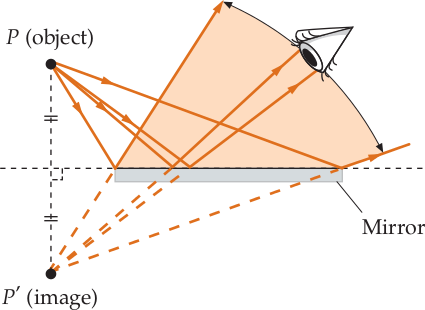
\includegraphics[width=0.5\textwidth]{images/4/41-mirall-pla.png}
\caption{Imatge formada per un mirall pla. Els rajos que venen del punt $P$ que van a parar al mirall sembla que vinguin del punt $P'$; es tracta d'una imatge virtual}
\end{figure}
Si fiques la mà dreta al davant d'un mirall, la imatge no és magnificada ni reduïda, però sembla una mà esquerra. Aquesta reversió dreta--esquerra és el resultat d'una \emph{inversió en profunditat}.

\subsubsection*{Exemples de miralls plans}
\begin{figure}[H]
\centering
    WIP: GRAFIC BONIC 
\caption{Periscopi}
\end{figure}

\begin{figure}[H]
\centering
    WIP: GRAFIC BONIC 
\caption{Caleidoscopi}
\end{figure}

\begin{figure}[H]
\centering
    WIP: GRAFIC BONIC 
\caption{Retroreflector}
\end{figure}

%----------------------------------------------------------------------------------------
\subsection{Miralls esfèrics}
Els miralls còncaus produeixen imatges reals i virtuals, mentre que els miralls convexos només produeixen de virtuals.
\begin{figure}[H]
\centering
    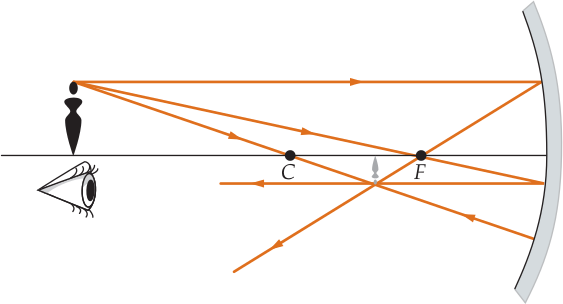
\includegraphics[width=0.6\textwidth]{images/4/42-mirall-esferic.png}
\caption{Imatge formada per un mirall esfèric. Els rajos que venen del punt $P$ que van a parar al mirall convergeixen en el punt $P'$; es tracta d'una imatge real}
\end{figure}

\subsubsection*{Diagrama de rajos per a miralls}
Dels infinits rajos, hi ha tres ---els rajos principals--- que són molt convenients d'emprar:
\begin{enumerate}
    \item Raig paral·lel: dibuixat paral·lel a l'eix. Aquest raig és reflectit al punt focal ($F$).
    \item Raig focal: dibuixat tal que passi pel punt focal ($F$). Aquest raig és reflectit paral·lel a l'eix.
    \item Raig radial: dibuixat tal que passi pel centre de curvatura ($C$). Aquest raig és reflectit en la mateixa direcció de provinença.
\end{enumerate}

La imatge es forma allà on convergeixen aquests tres rajos.

\subsubsection*{Convenció de signes}
\begin{enumerate}
    \item $s$ és positiva si l'objecte està a la banda de la llum incident del mirall.
    \item $s'$ és positiva si la imatge es forma a la banda de la llum reflectida del mirall.
    \item $r$ (i, per tant, $f$) és positiva si el mirall és còncau, de manera que el centre de curvatura està a la banda de la llum reflectida del mirall.
\end{enumerate}
Assumint que tots els rajos són paraxials (aproximadament paral·lels a l'eix), podem establir la següent relació:
\begin{align}
    \boxed{\frac{1}{s} + \frac{1}{s'} = \frac{2}{r}} \label{eq:miralls1}
\end{align}
Es pot establir una relació entre les llargades dels objectes i les seves posicions, que anomenem magnificació lateral de la imatge:
\begin{align}
    \boxed{m = \frac{y'}{y} = - \frac{s'}{s}}
\end{align}
Quan els rajos venen de l'infinit, la imatge es forma al punt focal $F$. La distància entre el mirall i aquest punt s'anomena distància focal i es defineix com a:
\begin{align}
    \boxed{f = \frac{1}{2} r}
\end{align}

Així doncs, podem reescriure l'equació \ref{eq:miralls1}, que anomenem equació dels miralls:
\begin{align}
    \boxed{\frac{1}{s} + \frac{1}{s'} = \frac{1}{f}} \label{eq:miralls2}
\end{align}

%----------------------------------------------------------------------------------------
\subsection{Lents}
\subsubsection*{Imatges formades per refracció}
\begin{figure}[H]
\centering
    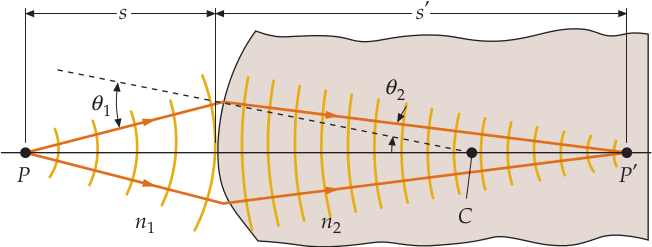
\includegraphics[width=0.8\textwidth]{images/4/43-refraccio.png}
\caption{Imatge formada per la refracció de la llum a una sola superfície esfèrica}
\end{figure}
\begin{align}
    \boxed{\frac{n_{1}}{s} + \frac{n_{2}}{s'} = \frac{n_{2} - n_{1}}{r}}
\end{align}
\subsubsection*{Convenció de signes}
\begin{enumerate}
    \item $s$ és positiva si l'objecte està a la banda de la llum incident de la superfície.
    \item $s'$ és positiva si la imatge es forma a la banda de la llum refractada de la superfície.
    \item $r$ és positiva si el centre de curvatura està a la banda de la llum refractada de la superfície.
\end{enumerate}
La magnificació causada per la refracció a una superfície esfèrica és:
\begin{align}
    \boxed{m = \frac{y'}{y} = - \frac{n_{1} s'}{n_{2} s}}
\end{align}

%----------------------------------------------------------------------------------------
\subsection{Lents primes}
\subsubsection*{Tipus de lents}
\begin{figure}[H]
\centering
    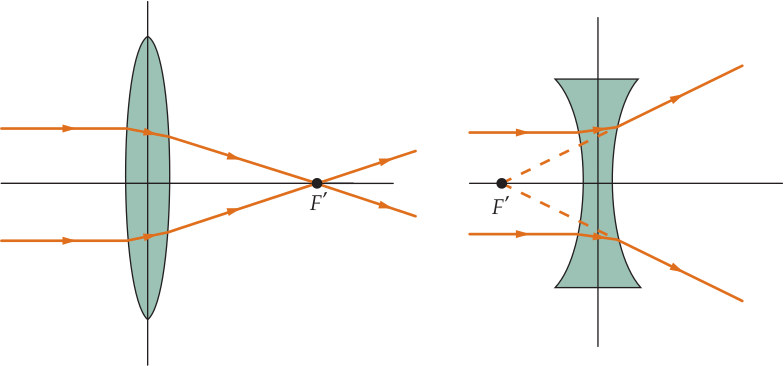
\includegraphics[width=0.9\textwidth]{images/4/44-conv-div.png}
\caption{Lents convergent i divergent, respectivament}
\end{figure}
\begin{figure}[H]
\centering
    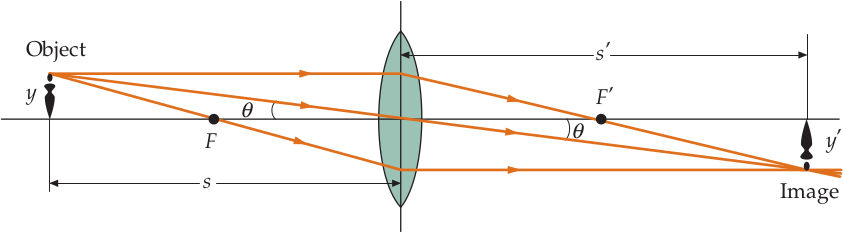
\includegraphics[width=\textwidth]{images/4/44-lents-primes.png}
\caption{Imatge formada per una lent prima convergent. Els rajos que venen del l'objecte van a parar a la lent i convergeixen formant una imatge real}
\end{figure}

\subsubsection*{Diagrama de rajos per a lents}
Dels infinits rajos, hi ha tres ---els rajos principals--- que són molt convenients d'emprar:
\begin{enumerate}
    \item Raig paral·lel: dibuixat paral·lel a l'eix. Aquest raig es dirigeix al segon punt focal de la lent ($F'$).
    \item Raig focal: dibuixat tal que passi pel primer punt focal ($F$). Aquest raig emergeix paral·lel a l'eix.
    \item Raig central: dibuixat tal que passi pel centre de la lent. Aquest raig no canvia la seva direcció\footnote{En realitat, les cares de les lents són paral·leles al centre, de manera que el raig emergeix en la mateixa direcció però desplaçat lleugerament. Com que la lent és prima, aquest fet és negligible.}.
\end{enumerate}
La imatge es forma allà on convergeixen aquests tres rajos.

L'equació creadora de lents és la següent:
\begin{align}
    \boxed{\frac{1}{f} = \left( \frac{n'}{n} - 1 \right) \left( \frac{1}{r_{1}} - \frac{1}{r_{2}} \right)}
\end{align}
L'equació de les lents primes és la mateixa que l'equació dels miralls \eqref{eq:miralls2}:
\begin{align}
    \boxed{\frac{1}{s} + \frac{1}{s'} = \frac{1}{f}}
\end{align}
La magnificació lateral d'una lent és:
\begin{align}
    \boxed{m = \frac{y'}{y} = - \frac{s'}{s}}
\end{align}

\subsubsection*{Potència d'una lent}
El recíproc de la distància focal s'anomena potència d'una lent. Quan la distància focal és expressada en metres, la potència s'expressa en diòptries ($D = \si{\per\m}$).
\begin{align}
    \boxed{P = \frac{1}{f}}
\end{align}

\subsubsection*{Combinació de lents}
Si tenim dues o més lents primes, podem trobar la imatge final produïda pel sistema cercant la distància de la imatge per a la primera lent i després utilitzant-la, juntament amb la distància entre les lents, per trobar la distància de l'objecte de la segona lent. És a dir, considerem cada imatge, si real o virtual ---i si és realment formada o no--- com a objecte per a la següent lent.
\begin{figure}
\centering
    WIP: GRAFIC BONIC 
\caption{Combinació de lents}
\end{figure}

\subsubsection*{Dues lents en contacte}
Quan tenim dues lents en contacte, la distància focal eficient és donada per la següent equació: 
\begin{align}
    \boxed{\frac{1}{f_{ef}} = \frac{1}{f_{1}} + \frac{1}{f_{2}}}
\end{align}
La potència eficient de dues lents en contacte és:
\begin{align}
    \boxed{P_{ef} = P_{1} + P_{2}}
\end{align}

%----------------------------------------------------------------------------------------
\subsection{Aberracions}
Quan tots els rajos des d'un objecte puntual no convergeixen en una única imatge puntual, el desenfocament resultant s'anomena aberració. 
\begin{figure}[H]
\centering
    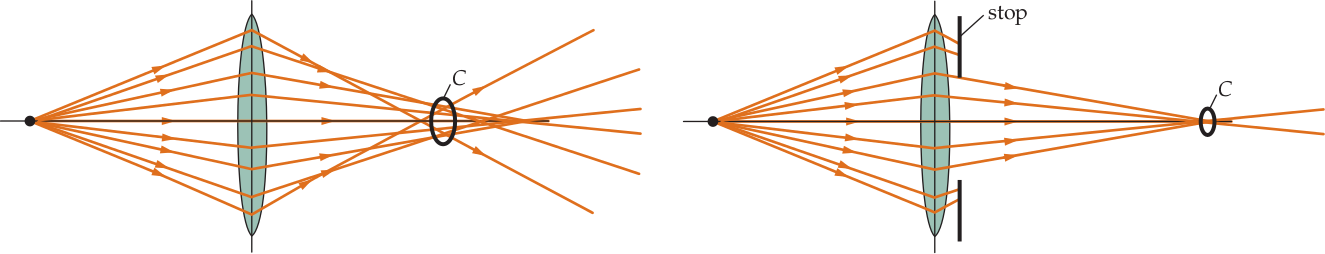
\includegraphics[width=\textwidth]{images/4/45-aberracions.png}
\caption{L'aberració esfèrica produïda per una lent es pot disminuir reduint l'obertura amb un diafragma.}
\end{figure}